\chapter{$L$-bounded cuts}

In this chapter we will consider a new problem which is length bounded cuts. This problem is NP-hard.

\begin{itemize}[]
	\item \textbf{INPUT} $G = (V,E)$, $s,t \in V$, $L \in \N$.
	\item \textbf{OUTPUT} $F \subseteq E$ such that $d_{G \setminus F}(s,t) > L$.
	\item \textbf{OBJECTIVE} $\min (|F|)$.
\end{itemize}

Lets see an easy example of a graph $G$ as shown on the picture \ref{l-bounded cut} and for $L = 4$. There can actually be two minimal $L$-bounded cuts. The \textcolor{orange}{first} one is actually not a "real" cut, but the \textcolor{cyan}{second} one is.

\begin{figure}[!ht]\centering
	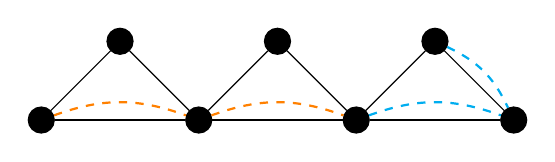
\begin{tikzpicture}[node distance={10mm}, main/.style = {draw, fill, circle}]
		\node[main] (1) {};
		\node[right of = 1] (1a) {};
		\node[main, above of = 1a] (1b) {};
		\node[main, right of = 1a] (2) {};
		\node[right of = 2] (2a) {};
		\node[main, above of = 2a] (2b) {};
		\node[main, right of = 2a] (3) {};
		\node[right of = 3] (3a) {};
		\node[main, above of = 3a] (3b) {};
		\node[main, right of = 3a] (4) {};
		
		\draw (1) edge (2);
		\draw (1) edge (1b);
		\draw (1b) edge (2);
		
		\draw (2) edge (3);
		\draw (2) edge (2b);
		\draw (2b) edge (3);
		
		\draw (3) edge (4);
		\draw (3) edge (3b);
		\draw (3b) edge (4);
		
		\draw[color = orange, thick, bend left = 20, dashed] (1) edge (2);
		\draw[color = orange, thick, bend left = 20, dashed] (2) edge (3);
		
		\draw[color = cyan, thick, bend left = 20, dashed] (3) edge (4);
		\draw[color = cyan, thick, bend left = 20, dashed] (3b) edge (4);
	\end{tikzpicture}
	\caption{Example of $L$-bounded cut. The cut is drawn by a multiple dashed edge.}
	\label{l-bounded cut}
\end{figure}


\section{$L$-bounded flow}

For $L$-bounded cut there is also the opposite problem which is in P and it is the $L$-bounded flow.

\begin{itemize}[]
	\item \textbf{INPUT} $G = (V,E)$, $s,t \in V$, $L \in \N$.
	\item \textbf{OUTPUT} Flow between $s-t$ that can be decomposed into paths of length $\leq L$.
	\item \textbf{OBJECTIVE} $\max$ the flow.
\end{itemize}

We will also show us an example for a graph $G$ depicted on the picture \ref{l-bounded flow} for $L = 3k$. We may see that $L$-cut is $k+1$ since we may delete \textcolor{cyan}{these edges} but also \textcolor{orange}{the bottom ones}. On the other hand $L$-flow is at most 2.

\begin{figure}[!ht]\centering
	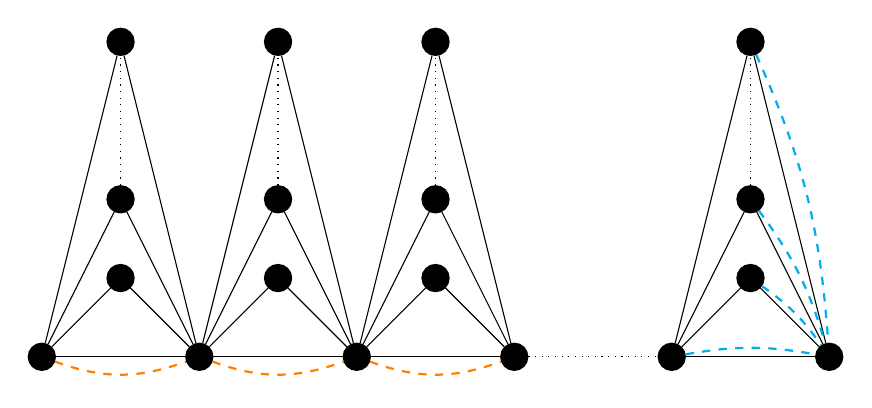
\begin{tikzpicture}[node distance={10mm}, main/.style = {draw, thick, fill, circle}]
		\node[main] (1) {};
		\node[right of = 1] (1a) {};
		\node[main, above of = 1a] (1b) {};
		
		\node[main, above of = 1b] (1c) {};
		\node[above of = 1c] (1d) {};
		\node[main, above of = 1d] (1e) {};
		
		\node[main, right of = 1a] (2) {};
		\node[right of = 2] (2a) {};
		\node[main, above of = 2a] (2b) {};
		
		\node[main, above of = 2b] (2c) {};
		\node[above of = 2c] (2d) {};
		\node[main, above of = 2d] (2e) {};
		
		\node[main, right of = 2a] (3) {};
		\node[right of = 3] (3a) {};
		\node[main, above of = 3a] (3b) {};
		
		\node[main, above of = 3b] (3c) {};
		\node[above of = 3c] (3d) {};
		\node[main, above of = 3d] (3e) {};
		
		\node[main, right of = 3a] (4) {};
		
		\node[right of = 4] (phantom) {};
		
		\node[main, right of = phantom] (k) {};
		\node[right of = k] (ka) {};
		\node[main, above of = ka] (kb) {};
		
		\node[main, above of = kb] (kc) {};
		\node[above of = kc] (kd) {};
		\node[main, above of = kd] (ke) {};
		
		\node[main, right of = ka] (k+1) {};
		
		\draw (1) edge (2);
		\draw (1) edge (1b);
		\draw (1b) edge (2);
		\draw (1) edge (1c);
		\draw (1c) edge (2);
		\draw (1) edge (1e);
		\draw (1e) edge (2);
		\draw[dotted] (1c) edge (1e);
		
		\draw (2) edge (3);
		\draw (2) edge (2b);
		\draw (2b) edge (3);
		\draw (2) edge (2c);
		\draw (2c) edge (3);
		\draw (2) edge (2e);
		\draw (2e) edge (3);
		\draw[dotted] (2c) edge (2e);
		
		\draw (3) edge (4);
		\draw (3) edge (3b);
		\draw (3b) edge (4);
		\draw (3) edge (3c);
		\draw (3c) edge (4);
		\draw (3) edge (3e);
		\draw (3e) edge (4);
		\draw[dotted] (3c) edge (3e);
		
		\draw[dotted] (4) edge (k);
		
		\draw (k) edge (k+1);
		\draw (k) edge (kb);
		\draw (kb) edge (k+1);
		\draw (k) edge (kc);
		\draw (kc) edge (k+1);
		\draw (k) edge (ke);
		\draw (ke) edge (k+1);
		\draw[dotted] (kc) edge (ke);
		
		\draw[dashed, thick, color = cyan, bend left = 10] (k) edge (k+1);
		\draw[dashed, thick, color = cyan, bend left = 10] (kb) edge (k+1);
		\draw[dashed, thick, color = cyan, bend left = 10] (kc) edge (k+1);
		\draw[dashed, thick, color = cyan, bend left = 10] (ke) edge (k+1);
		
		\draw[dashed, thick, color = orange, bend right = 20] (1) edge (2);
		\draw[dashed, thick, color = orange, bend right = 20] (2) edge (3);
		\draw[dashed, thick, color = orange, bend right = 20] (3) edge (4);
	\end{tikzpicture}
	\caption{Example of $L$-bounded flow. Where there is $2k$ bottom vertices and $k$ upwards in each triangle. Cuts are represented by multi edges that are dashed.}
	\label{l-bounded flow}
\end{figure}

\begin{observ}
	Every $L$-bounded $s-t$ path uses at least $k$-edges from the bottom so max $L$-flow is at most 2.
\end{observ}

Therefore the difference between $L$-cut and $L$-flow can be at least $\sqrt{n}$.

\section{Approximation for $L$-cut}

Consider the following LP relaxation (denoted as (\textbf{D})). Alternatively the ILP will surely solve the problem. Lets denote $\mathcal{P}_L$ as the set of all $L$-bounded $s-t$ paths.

$$
\begin{aligned}
	\min \sum_{e \in E} x_e & \\
	\sum_{x \in p} x_e \geq 1 & \quad \forall p \in \mathcal{P}_L \\
	x_e \geq 0 & \quad \forall e \in E
\end{aligned}
$$

Also we can see what is the is the dual to this LP. Which will indeed solve $L$-flows. And we will denote it as (\textbf{P}).

$$
\begin{aligned}
	\max \sum_{p \in \mathcal{P}_L} f_p &\\
	\sum_{p: e \in p \in \mathcal{P}_L} f_p \leq 1 & \quad \forall e \in E\\
	f_p \geq 0 & \quad \forall p \in \mathcal{P}_L
\end{aligned}
$$

We may ask ourselves what is the integrality gap? From the instance shown on the picture \ref{l-bounded flow} we already saw that the max $L$-flow is $2$ and min $L$-cut is about $c \sqrt{n}$. Because of the duality we know the $L$-flow is the same as fractional $L$-cut, therefore the integrality gap is $\geq \Omega (\sqrt{n})$.

\subsection{$L$-approximations}

We can create multiple quite simple algorithms for solving such problem. These all will be approximation algorithms.

\begin{algorithm}
	\caption{ \texttt{(1)} $L$-bounded cut approximation}
	\begin{algorithmic}[1]
		\Require $G = (V,E)$
		\Ensure $L$-bounded cut.
		\While{$\exists L$-bounded $s-t$ path $p$ in $G$}
			\State Remove all edges of $p$.
		\EndWhile
	\end{algorithmic}
\end{algorithm}

\begin{observ}
	While the OPT $\geq k$ therefore it is $L$-approximation. Since the $k$ is the number of $L$-paths.
\end{observ}

\begin{algorithm}
	\caption{ \texttt{(2)} $L$-bounded cut approximation}
	\begin{algorithmic}[1]
		\Require $G = (V,E)$
		\Ensure $L$-bounded cut.
		\While{$d_g(s,t) \leq L$}
			\State $F := $ min cut in a subgraph of shortest paths.
			\State $G = G \setminus F$
		\EndWhile
	\end{algorithmic}
\end{algorithm}

We may clearly see that $|F| \leq \text{opt } L-\text{cut}$. Because we always need to delete some of these edges. We also always increase the shortest path by 1. Therefore it is an $L$-approximation since it is at max $L$ steps in the algorithm and for each it is at most the optimum.

\begin{algorithm}
	\caption{ \texttt{(3)} $L$-bounded cut approximation}
	\begin{algorithmic}[1]
		\Require $G = (V,E)$
		\Ensure $L$-bounded cut.
		\State Solve (\textbf{P}).
		\State $F := \{e \in E: \sum_{p : e \in p} f_p = 1\}$
	\end{algorithmic}
\end{algorithm}

In other words all saturated edges will form the $L$-cut. Now if $F$ wouldn't be an $L$-cut then the maximal flow was not maximal, since there is an $L$-path with non-saturated edge. Also $|F| \leq L (\max L-\text{flow})$ that is because every unit of a flow can saturate at most $L$ edges. And due to the duality $|F| \leq L (\max L-\text{flow}) \leq L (\min L-\text{cut})$. So once more we have obtained $L$-approximation.

\begin{algorithm}
	\caption{ \texttt{(4)} $L$-bounded cut approximation}
	\begin{algorithmic}[1]
		\Require $G = (V,E)$
		\Ensure $L$-bounded cut.
		\State Solve (\textbf{D}).
		\State $F := \left\{e \in E: x_e \geq \frac{1}{L}\right\}$
	\end{algorithmic}
\end{algorithm}

Due to the pigeonhole principle at least one edge in $L$-path has to have $\frac{1}{L}$, therefore it is a feasible solution. Because we are scaling the solution by the $L$ fraction we may see that $|F| \leq L (\min \text{ fractional } L-\text{cut}) \leq L \cdot \text{OPT}$. So we have another $L$-approximation.

There is an somewhat easy $L/2$-approximation only by combining \texttt{(1)} and \texttt{(2)}. This start with \texttt{(1)} with the bond lowered to $L/2$, then we switch to \texttt{(2)}.

\subsection{$n^{2/3}$-approximations}

Now what if we want to get approximation based on $n = |V(G)|$ instead of $L$. Can we create a $(n^{2/3})$-approximation. Firstly if $L \leq n^{2/3}$ then we are done by running $L$-approximation.

Otherwise we denote $\text{OPT}_L$ as the size of the optimal min $L$-cut. We may observe that for $L' < L$ it holds that $\text{OPT}_{L'} \leq \text{OPT}_L$ because all $L'$-paths are also $L$-paths.

The algorithm would be as follows. Firstly run $(n^{2/3})$-approximation from one of the four algorithms for this parameter. This will cost $O(n^{2/3} \cdot \text{OPT}_L)$.

Then by the theorem \ref{max flow bounded} we get that $l = n^{2/3}$ so the max flow is $\leq O(n^{2/3})$. Thus we can run the basic min cut problem on the whole graph which will also cost $O(n^{2/3} \cdot \text{OPT}_L)$ and also all together will be the same cost asymptotically.

\section{Integrality gap}

We will now create an instance for $L$-cut that has an integrality gap $n^{2/3}$. The scheme of the instance is depicted on picture \ref{huge integrality gap}. Firstly from $s$ node there are $n^{2/3}$ neighbors in the second layer. Next from the \textcolor{violet}{consecutive $n^{1/3}$ nodes} in the second layer have one common neighbor in the third layer. Therefore there is $n^{1/3}$ nodes in the third layer. After that it repeats for $n^{2/3}$ next layers and these middle parts form a \textcolor{cyan}{complete bipartite graph}. Then the last layer before $t$ is the same as from $s$, so it is a mirror image.

This is the underline structure where we add a \textcolor{orange}{shortcut} that skips every second layer. And lets say that there is $2k$ of the shortcuts.

\begin{figure}[!ht]\centering
	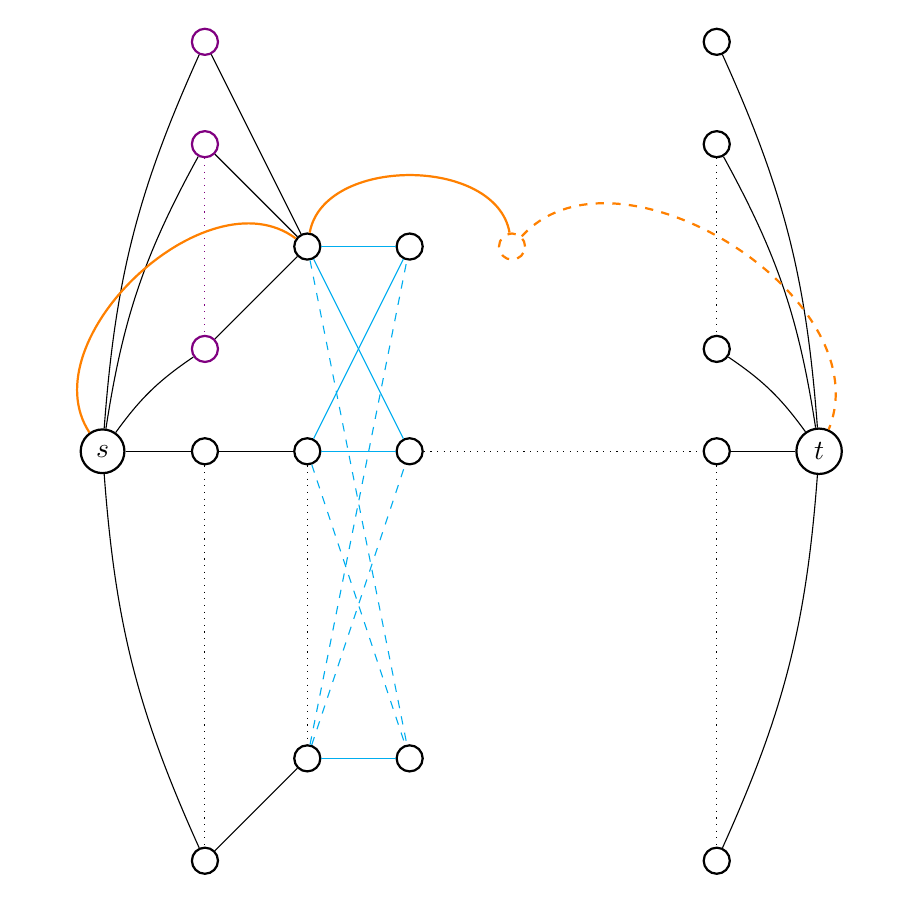
\begin{tikzpicture}[node distance={13mm}, main/.style = {draw, thick, circle}]
		%% Nodes
		\node[main] (s) {$s$};
		% First layer.
		\node[main, right of = s] (2) {};
		\node[main, above of = 2, color = violet] (1l) {};
		\node[above of = 1l] (1phantom) {};
		\node[main, above of = 1phantom, color = violet] (12) {};
		\node[main, above of = 12, color = violet] (11) {};
		\node[below of = 2] (ph1) {};
		\node[below of = ph1] (ph2) {};
		\node[below of = ph2] (ph3) {};
		\node[main, below of = ph3] (last) {};
		% Second layer.
		\node[main, right of = 2] (3) {};
		\node[above of = 3] (ph-layer2-3) {};
		\node[main, above of = ph-layer2-3] (layer21) {};
		\node[below of = 3] (ph-layer2-4) {};
		\node[below of = ph-layer2-4] (ph-layer2-5) {};
		\node[main, below of = ph-layer2-5] (layer2last) {};
		% Third layer.
		\node[main, right of = 3] (4) {};
		\node[main, right of = layer21] (layer31) {};
		\node[main, right of = layer2last] (layer3last) {};
		% Shortcut 4 layer.
		\node[main, dashed, color = orange, right of = layer31] (shortcut) {};
		% Mid layers.
		\node[right of = 4] (5) {};
		\node[right of = 5] (6) {};
		% Last layer.
		\node[main, right of = 6] (7) {};
		\node[main, above of = 7] (7l) {};
		\node[above of = 7l] (7phantom) {};
		\node[main, above of = 7phantom] (72) {};
		\node[main, above of = 72] (71) {};
		\node[below of = 7] (ph7) {};
		\node[below of = ph7] (ph8) {};
		\node[below of = ph8] (ph9) {};
		\node[main, below of = ph9] (last7) {};
		\node[main, right of = 7] (t) {$t$};
		%% Edges.
		\draw (s) edge (2);
		\draw[bend left = 10] (s) edge (11);
		\draw[bend left = 10] (s) edge (12);
		\draw[bend left = 10] (s) edge (1l);
		\draw[bend right = 10] (s) edge (last);
		% Dots.
		\draw[dotted, color = violet] (12) edge (1l);
		\draw[dotted] (2) edge (last);
		% Second layer.
		\draw (2) edge (3);
		\draw (11) edge (layer21);
		\draw (12) edge (layer21);
		\draw (1l) edge (layer21);
		\draw (last) edge (layer2last);
		% Dots.
		\draw[dotted] (3) edge (layer2last);
		% Third layer.
		\draw[color = cyan] (layer21) edge (layer31);
		\draw[color = cyan] (3) edge (layer31);
		\draw[dashed, color = cyan] (layer2last) edge (layer31);
		\draw[dashed, color = cyan] (layer21) edge (layer3last);
		\draw[dashed, color = cyan] (3) edge (layer3last);
		\draw[color = cyan] (layer2last) edge (layer3last);
		\draw[color = cyan] (layer21) edge (4);
		\draw[color = cyan] (3) edge (4);
		\draw[dashed, color = cyan] (layer2last) edge (4);
		% Dots.
		\draw[dotted] (4) edge (7);
		% Last layer.
		\draw (t) edge (7);
		\draw[bend left = 10] (71) edge (t);
		\draw[bend left = 10] (72) edge (t);
		\draw[bend left = 10] (7l) edge (t);
		\draw[bend right = 10] (last7) edge (t);
		% Dots.
		\draw[dotted] (72) edge (7l);
		\draw[dotted] (7) edge (last7);
		% Shortcut.
		\draw[color = orange, bend left = 80, thick] (s) edge (layer21);
		\draw[color = orange, bend left = 80, thick] (layer21) edge (shortcut);
		\draw[color = orange, bend left = 80, thick, dashed] (shortcut) edge (t);
	\end{tikzpicture}
	\caption{Instance of an $L$-cut with integrality gap $n^{2/3}$.}
	\label{huge integrality gap}
\end{figure}

Let $L = 3k$. As in the previous instance at least half of (that is $k$) the shortcut must be used for $L$-flow. Hence the max $L$-flow is at most 2. But one can prove that the following holds. Min $L$-cut is at least $n^{2/3}$. That is we can remove edges between two parts that form complete bipartite graph. This is only a sketch and it does not get into a details.

All in all this particular instance has integrality gap $O(n^{2/3})$.

\section{$L$-flow}

In this section we will take a look at an algorithm for $L$-flow that would be fast and won't used \textbf{LP}. As it turns out there is as of now only an approximation scheme, which is fully polynomial time approximation scheme (FPTAS for short). Now $y(e)$ is the value for min cut in (\textbf{D}) and $c(e)$ the capacity for edge $e$. Then $x(p)$ is the same as $f_p$ in (\textbf{P}).

\begin{algorithm}
	\caption{FPTAS for $\max L$-flow}
	\begin{algorithmic}[1]
		\Require $G = (V,E)$
		\Ensure $\max L$-bounded flow.
		\State $\epsilon > 0$ $\forall e \in E$, $\delta = \delta(\epsilon)$ $\forall p \in \mathcal{P}_L$
		\While{the $y$-shortest path $p \in \mathcal{P}_L$ has length $< 1$}
			\State $c = \min_{e \in p} c(e)$
			\State $x(p) = x(p) + \epsilon$
			\State $y(e) = y(e) \left( 1 + \frac{\epsilon c}{c(e)} \right)$ $\forall e \in p$
		\EndWhile
		\State \Return $x$
	\end{algorithmic}
\end{algorithm}

\begin{lemma}
	$x$ scaled down by $\log_{1 + \epsilon} \frac{1+\epsilon}{\delta}$ is a feasible solution.
\end{lemma}

\begin{thm}
	The scaled flow is $(1 + \epsilon)$-approximation.
\end{thm}

Few remarks. Firstly this algorithm can be done by using Dijkstra's algorithm on the layered graph, which is similiar to the one already mentioned. That is $L$ layers and finding shortest path from $(s,0)$ to $(t, L)$. Other remark is that indeed this does not use LP.

Sometimes this type of algorithm is called \textit{Multiplicative weight update algorithm}. Which can also be applied for the multi-commodity flow. Intuitively the algorithm avoids heavily used edges and prefer spreading the flows.